\chapter{Análisis del estado del arte}
\label{cap:estado_del_arte}


 


% En Español: 
\section{Introducción}

% En Ingles: 
%\section{INTRODUCTION}
\par
La implementación de sistemas de control de supervisión y adquisición de datos (\ac{SCADA}) constituye un elemento esencial dentro de los procesos de automatización industrial, ya que permite no solo recopilar y archivar información, sino también visualizarla, transmitirla y gestionarla de manera eficiente, asegurando así un control integral de las operaciones. En el ámbito de la generación eléctrica, estos sistemas se han consolidado como herramientas imprescindibles para optimizar tanto la eficiencia como el mantenimiento de grandes aerogeneradores, además de facilitar la gestión de las subestaciones eléctricas asociadas. A partir de los avances alcanzados en los últimos años, la investigación académica ha orientado sus esfuerzos hacia la mejora de la eficiencia en la producción energética y la resolución de los problemas derivados de la creciente descentralización de los sistemas de generación.\par


\subsection{Arquitecturas inalámbricas en parques eólicos}
Un enfoque de creciente interés dentro del estado del arte se centra en la flexibilización y modernización de la infraestructura de comunicaciones mediante el despliegue de redes inalámbricas bajo el paradigma de los Sistemas Ciberfísicos (CPS). Autores como Ahmed et al. \cite{Ahmed2020} \cite{ahmed2014communication} defienden que las soluciones inalámbricas estructuradas de forma jerárquica y basadas en el estándar IEC 61400-25 segmentando el tráfico en redes internas de la turbina (WTIN), perimetrales (WTAN) y globales del parque (WFAN) superan las limitaciones de los sistemas convencionales cableados al reducir drásticamente los costes de instalación y ofrecer topologías dinámicas y escalables, especialmente viables en entornos remotos o de orografía compleja \cite{gungor2009industrial}. En sus investigaciones, mediante simulaciones de flujos de datos analógicos de alta frecuencia, demuestran que tecnologías como Wi-Fi y ethernet no solo son viables, sino que logran cumplir con los estrictos requisitos de retardo extremo a extremo, relegando a tecnologías de bajo ancho de banda como ZigBee a telemetrías secundarias\cite{mahmood2015review}.\par  

\begin{figure}[tb]
    \begin{subfigure}{0.3\textwidth}
        \centering
        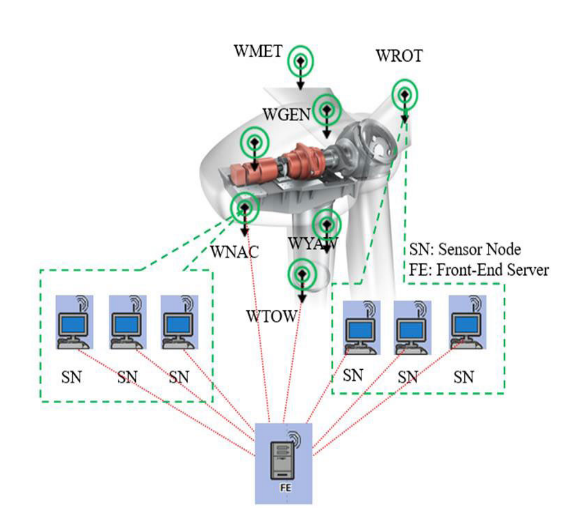
\includegraphics[width=\textwidth,height=0.8\linewidth]{figuras/Wifi.png}
        \caption{Arquitectura de red inalámbrica en parques eólicos.}
        \label{fig:wifi}
    \end{subfigure}
     \begin{subfigure}{0.3\textwidth}
        \centering
        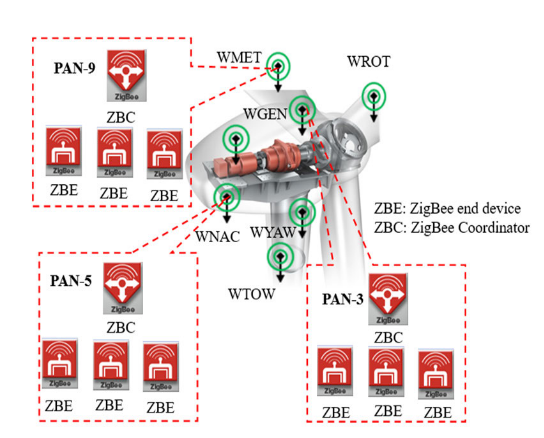
\includegraphics[width=\textwidth,height=0.8\linewidth]{figuras/zigbee.png}
        \caption{Arquitectura de red inalámbrica ZigBee en parques eólicos.}
        \label{fig:zigbee}
    \end{subfigure}
    \begin{subfigure}{0.3\textwidth}
        \centering
        \includegraphics[width=\textwidth,height=0.8\linewidth]{figuras/ethernet.png}
        \caption{Arquitectura de red cableada con ethernet en parques eólicos.}
        \label{fig:ethernet}
    \end{subfigure}
    \caption{Comparativa de arquitecturas inalámbricas en aerogeneradores. Obtenido de \cite{Ahmed2020}}
\end{figure}

Sin embargo, desde una perspectiva de operación crítica en el sector eléctrico, las tecnologías inalámbricas introducen incertidumbres asociadas a la pérdida de determinismo y la vulnerabilidad ante interferencias electromagnéticas severas, habituales en el entorno perimetral de un aerogenerador.\par

\subsection{Ciberseguridad en sistemas \ac{SCADA} de parques eólicos}
Por otra parte, la creciente necesidad de interoperabilidad entre sistemas empuja a que los \ac{SCADA} se diseñen para facilitar el acceso externo a la información sin comprometer la seguridad operativa. En lo que respecta a la exposición segura de variables operacionales hacia el exterior, el estado del arte marca la importancia de la segmentación de red en infraestructuras eólicas distribuidas. Autores como Shih abordan este desafío en entornos de parques eólicos marinos mediante el despliegue de \ac{DMZ} combinadas con el protocolo de telecontrol IEC 60870-5-104 \cite{Shih2022}. La arquitectura de Shih demuestra que interponer una \ac{DMZ} resguarda eficazmente la red local de control \ac{OT} frente a intrusiones externas, permitiendo que terceras entidades consulten históricos de viento y generación sin comprometer la estabilidad de los activos.\par

No obstante, el despliegue de una \ac{DMZ} local compleja requiere servidores e infraestructura de red replicada en planta para aislar el tráfico. En lugar de ello se puede utilizar el protocolo \ac{MQTT} nativo desde un \ac{SCADA} debido a su naturaleza unidireccional y basada en publicaciones y de poca latencia \cite{ferrari2020evaluation}. Con \ac{MQTT}, es el propio nodo perimetral de la planta (Edge) el que abre de forma segura una única conexión saliente \ac{TCP} hacia un bróker en la nube para publicar los datos. Al no requerir puertos de entrada abiertos en la red local de operaciones (OT), se elimina superficie para un ciberataque, simplificando la arquitectura de ciberseguridad sin perder visibilidad.\par

\subsection{Mantenimiento predictivo y predicción de potencia mediante inteligencia artificial}
Más allá de la transmisión de datos, uno de los retos más relevantes en la gestión de parques eólicos es la predicción de la potencia generada. Tradicionalmente, esta se estima mediante curvas de potencia obtenidas a partir de técnicas de reducción de datos como el \textit{binning}, en el que se agrupan las velocidades de viento y las densidades del aire en intervalos específicos. Sin embargo, el aumento en el tamaño de las turbinas hace que fenómenos como la cizalladura del viento o la intensidad de las turbulencias tengan un impacto mayor en la curva, al utilizar datos históricos meteorológicos recopilados por un sistema \ac{SCADA} se pueden mejorar significativamente las predicciones clásicas \cite{Pandit2023}.

El mantenimiento predictivo se ha consolidado como uno de los principales beneficios de los sistemas \ac{SCADA}, ya que permite anticipar fallos, reducir costes operativos y garantizar la seguridad tanto de los trabajadores como de las infraestructuras, por ejemplo, tras el impacto de un rayo en una pala de aerogenerador para determinar el grado de daño \cite{Matsui2021}. También se puede utilizar para la predicción de fallos por desgaste y en la construcción de modelos de diagnóstico basados íntegramente en datos de salud de aerogeneradores \cite{Khan2024} \cite{Shi2021}.

En terrenos muy complejos, asumir que todas las turbinas sufren las mismas condiciones ambientales no es realista ya que varían significativamente entre turbinas. Los métodos tradicionales confunden estas variaciones (o paradas manuales) con fallos mecánicos. Por ello, existen soluciones dónde en lugar de agrupar todas las turbinas o un grupo menor por distancia física, se agrupan por similitud en condiciones externas. En estas soluciones, El \ac{SCADA} proporciona las variables ambientales críticas al algoritmo de clasificación necesarias para agrupar las turbinas correctamente, lo que ayuda a detectar fallos graves con meses de antelación sin generar falsas alarmas (ver figura \ref{fig:ml}), incluso en parques eólicos con orografía difícil \cite{Du2023}.

\begin{figure}[tb]
    \centering
    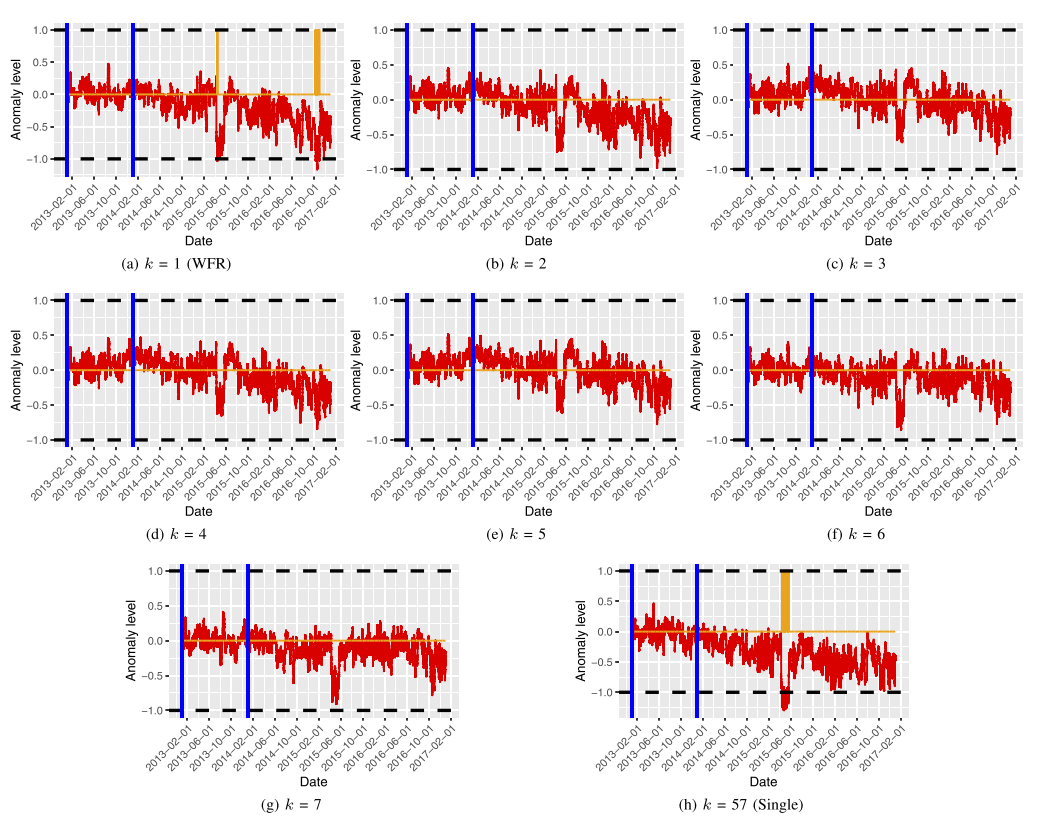
\includegraphics[width=\textwidth]{figuras/Anomalia.png}
    \caption{Evolucion de las falsas alarmas (naranja) en un parque eolico agrupando los aerogeneradores en grupos de condiciones (k-means) en lugar de por proximidad física \cite{Du2023}.}
    \label{fig:ml}
\end{figure}

Finalmente, la irrupción de las tecnologías de aprendizaje automático y profundo ha ampliado de manera significativa las posibilidades del mantenimiento predictivo. Algunos estudios emplean arquitecturas de \ac{CNN} para extraer patrones dinámicos de los datos de turbinas \cite{Kong2020} \cite{Xiang2021}, mientras que otros exploran modelos LSTM y regresiones para anticipar fallos en las curvas de potencia \cite{Udo2021}. Sin embargo, su efectividad depende intrínsecamente de la arquitectura de supervisión que se encarga de recoger los datos. Lo que revaloriza el diseño del sistema \ac{SCADA} como la infraestructura crítica e indispensable. Solo mediante un sistema de adquisición de calidad es posible alimentar estos algoritmos para optimizar la vida útil de los componentes, reducir costes y mejorar la fiabilidad del sistema.\par

\section{Conclusiones del estado del arte}
En conclusión, la eficacia de las técnicas avanzadas de predicción y mantenimiento dependen intrínsecamente de la calidad de la adquisición de datos. Esta base es el pilar de la gestión eficiente de parques eólicos, en las que tecnologías como la \ac{IA} y el \ac{ML} se sustentan para obtener predicciones precisas. Por todo esto, el desarrollo de un sistema de supervisión y adquisición de datos (\ac{SCADA}) eficiente, robusto y ciberseguro capaz además de alimentarse de plantas en cualquier entorno es indispensable para desarrollar e implementar las tecnologías emergentes para el mantenimiento predictivo del futuro, junto con las necesidades del sector energético. Lo que motiva el trabajo desarrollado en este TFM. \par
